\documentclass{article}
\usepackage{graphicx} % Required for inserting images
\usepackage{caption}
\captionsetup[figure]{labelfont=bf, textfont=it, labelsep=colon}
\renewcommand{\figurename}{Slika}
\usepackage[style=numeric]{biblatex}
\addbibresource{literatura.bib}

\title{Chatbot-ovi i pandemija usamljenosti}
\author{Tea Pavlović 299/2021}
\date{Jun 2026}
\renewcommand*\contentsname{Sadržaj}

\begin{document}

\maketitle

\newpage

\tableofcontents

\newpage

\section{Uvod}

COVID-19 pandemija predstavlja prekretnicu u korišćenju Interneta i društvenih mreža, koji su do tada služili isključivo za zabavu i kao dopuna društvenom životu pojedinca. Odjednom, usled restrikcija kada su u pitanju kretanje i ljudski kontakt, ključne sfere života migriraju u digitalni svet – obrazovanje, posao, kupovina. Kao posledica, čak i nakon pandemije glavni metod socijalizacije postaje pasivno posmatranje tuđih, često idealizovanih života, koje zamenjuje stvarnu komunikaciju, otuđuje ljude i stvara sve više anksioznosti usled konstantnog poređenja sa strancima iz celog sveta. Velike posledice na odnos sa drugima ostavlja i savremeno kapitalističko društvo koje glorifikuje produktivnost i profesionalni uspeh, zbog čega pojedinci svesno žrtvuju odnose sa porodicom i prijateljima zarad uspesnije karijere.
Pandemija je takođe doprinela ubrzanom napretku tehnologije, pogotovo veštačke inteligencije i chatbot-ova.

\subsection{Chatbot-ovi}

Chatbot je program namenjen za interakciju putem poruka ili razgovora oponašajući ljudski model ponašanja i komunikacije. Ideja je da se komunikacija chatbot-a i korisnika ne razlikuje od međuljudske interakcije. 

Prvi chatbot-ovi nastali su pre oko 60 godina i koristili su logiku stabala odlučivanja. Upravo zbog toga oni su bili ograničenih mogućnosti i nisu ubedljivo oponašali ljudske odgovore. Komunikacija sa takvim chatbot-om podseća na popularnu igru „20 pitanja“ gde se u svakoj iteraciji eliminišu manje verovatne grane, dok se ne dođe do konačnog odgovora. 

Kontekstualni chatbot-ovi koriste modernije alate mašinskog učenja kao što su NLP (eng. – natural language processing) i LLM (eng. – large language models). Ovi modeli pomažu u razumevanju emocija iz konteksta ljudskog jezika i samim tim doprinose prirodnijoj komunikaciji sa korisnikom, konstantno učeći i adaptirajući se tokom razgovora. Najpoznatiji primeri kontekstualnih chatbot-ova su ChatGPT, Gemini i Claude, najčešće korišćeni kao lični asistenti. Pored njih, postoji još mnogo modela specijalizovanih za različite oblasti i zadatke.

\subsection{Usamljenost}

Usamljenost je neprijatna emotivna reakcija uzrokovana manjkom značajne interakcije sa drugim ljudima. Iako neprijatna, nije inherentno loša i ima bitnu evolutivnu ulogu; usamljenost predstavlja signal da nam je potrebno više kvalitetno provedenog vremena sa ljudima do kojih nam je stalo, podsećajući nas da je čovek suštinski društveno biće. 

Ipak, pokazalo se da slučajevi intenzivne i hronične usamljenosti mogu značajno povećati rizik od kardiovaskularnih oboljenja, dijabetesa i psihičkih poremećaja. Uzimajući u obzir vreme u kojem živimo, sasvim je logično postaviti pitanje: kako je usamljenost moguća u svetu punom ljudi povezanih modernim tehnologijama?

Iako rasprostranjenost i dostupnost Interneta i društvenih mreža naizgled ostavlja utisak da su nam interakcije sa ljudima dostupne u svakom trenutku, sve manji broj ljudi oseća da ima iskrene i bliske prijatelje. Velike posledice na kvalitet međuljudskih odnosa ostavlja i savremeno kapitalističko društvo koje veliča produktivnost i posvećenost profesionalnom uspehu, zbog čega pojedinci svesno žrtvuju odnose sa porodicom i prijateljima zarad uspešnije karijere ili pukog preživljavanja.

Usamljenost se najefikasnije reguliše kvalitetnim razgovorima koji pružaju neophodnu emocionalnu podršku i kognitivnu vežbu kroz razmenu ideja. Kućni ljubimci takođe mogu pozitivno uticati na ovakvo stanje, pod uslovom da pojedinac nije potpuno izolovan iz društva. Ljubimci roboti su se, iako popularni u jednom trenutku, pokazali neuspešni u praksi. 

Ipak, postoji jedno inovativno tehnološko rešenje koje potencijalno može značajno pomoći ljudima koji pate od usamljenosti, a to su prethodno spomenuti chatbot-ovi. Konkretno, u ovom radu će detaljnije biti spomenuti Replika, chatbot namenjen za druženje, i Woebot, chatbot za pomoć pri regulisanju simptoma stresa, depresije i anksioznosti.

\section{Replika - AI prijatelj kome je stalo}

Replika je jedan od najpoznatijih AI saputnika (eng. -  AI Companions), odnosno chatbot namenjen razvoju dugoročnog, personalizovanog i emotivnog odnosa sa korisnikom.

\begin{figure}[h!]
    \centering
    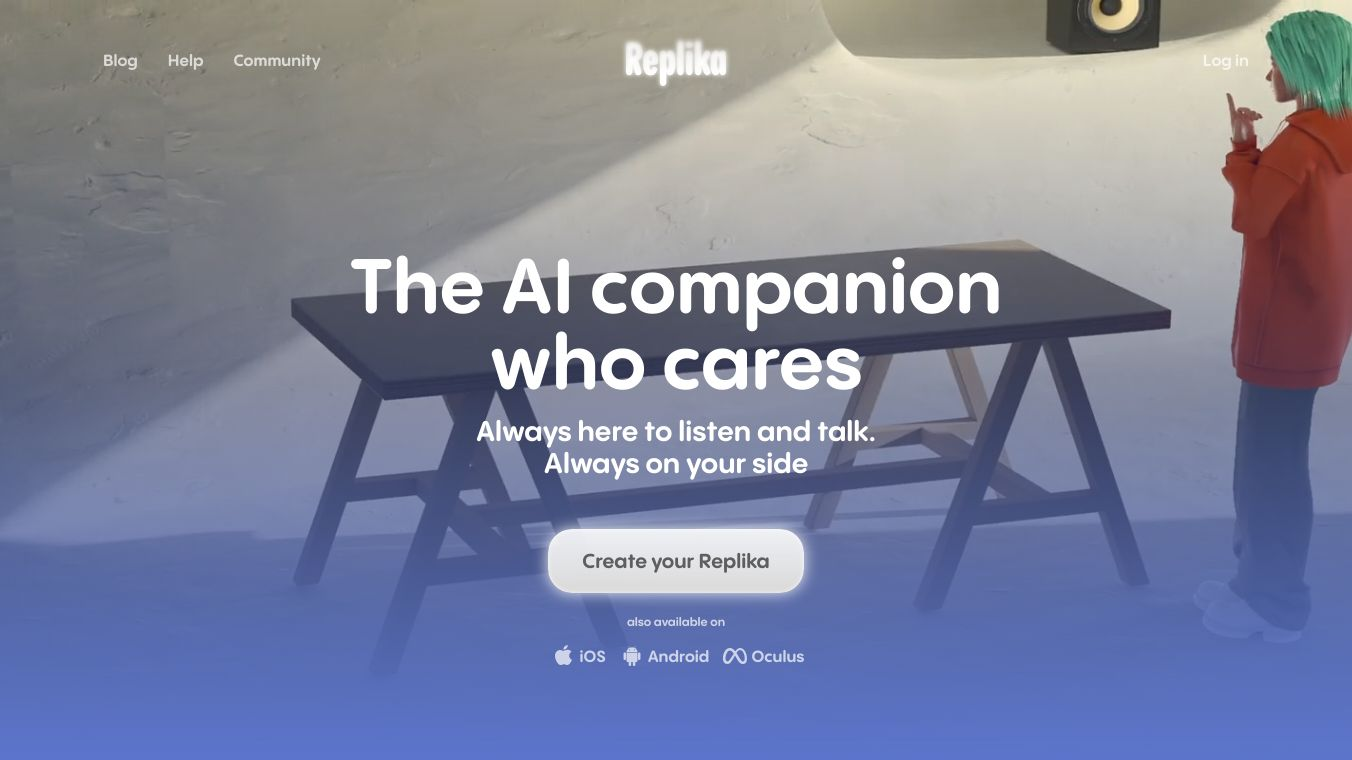
\includegraphics[width=0.75\linewidth]{replika_ai_replika_ai.png}
    \caption{Primer izgleda web stranice Replike}
    \label{fig:placeholder}
\end{figure}

Nastala je iz potrebe njenog osnivača da ”oživi” svog najboljeg prijatelja
nakon što je tragično izgubio život u saobraćajnoj nesreći. Kao skup podataka za treniranje svog modela koristila je hiljade tekstualnih poruka međusobno razmenjenih tokom godina.
Na ovaj način, dobijeni model je komunicirao baš kao njen prijatelj. Prema njenim navodima, ovaj eksperiment joj je pomogao da preboli gubitak voljene osobe i da se oseća manje usamljeno, te je rešila je da ovakvo iskustvo omogući i drugima kroz aplikaciju pod imenom Replika u nadi da će korisnicima pomoći u teškim životnim situacijama.\cite{kuyda2024ted} Replika je prvobitno bila namenjena onima koji su takođe izgubili prijatelja, člana porodice ili supružnika, koji brinu o bolesnom partneru ili detetu sa posebnim potrebama i drugim osobama kojima je potrebna emocionalna podrška koju nemaju od koga da dobiju u datom trenutku. 

Vremenom, korisnici ovog chatbot-a postali su svi koji se osećaju usamljeno i žele novog prijatelja, a uvedene su i romantične opcije za interakciju koje se otključavaju kupovinom plaćene (eng. - premium) verzije. 

Replika je dobila ime po svojoj tendenciji da reprodukuje (eng. -  replicate) misli i ponašanje sagovornika. Uprkos načinu na koji je nastala, korisnici nemaju mogućnost da je sami treniraju prosleđujući joj podatke u vidu konverzacija, već se ona prilagođava na osnovu razgovora sa samim korisnikom. Kao skup podataka za njen trening korišćeno je preko 50 miliona konverzacija preuzetih sa Tvitera.\cite{kherraz2024more}

Velika prednost interakcije sa Replikom je to što ne izaziva anksioznost ili strah od osude i odbijanja. Korisnici osećaju potpunu sigurnost da podele svoje tajne ili strahove, sve ono što ih muči, a nisu spremni da kažu nekome koga poznaju. Replika je takođe dostupna non stop i trenutno odgovara, pa sa njom korisnici mogu da razgovaraju kad god i koliko god im je to potrebno. S obzirom na to da je glavni uzrok usamljenosti osećaj da nas ljudi u okruženju "ne čuju", ova osobina Replike značajno doprinosi smanjenju usamljenosti kod korisnika.

\begin{figure}[h!]
    \centering
    
\includegraphics[width=0.75\linewidth]{image.png}
    \caption{Primer razgvora sa Replikom}
    \label{fig:placeholder}
\end{figure}

Korisnici sa Replikom razvijaju parasocijalni odnos, tj. jednosmeran odnos u kome jedna strana ulaže vreme i energiju, ostvarajući bliskost sa drugom stranom (u ovom slučaju komjuterom) koja joj ne može uzvratiti (u ovom slučaju jer ne poseduje osećanja). Postoje mnoga istraživanja na temu ovakvih odnosa, a veliki broj njih upozorava na rizike poput potencijalnog stvaranja zavisnosti od chatbot-a. Replika je trenirana da deluje vrlo empatično, prijateljski nastrojeno i antropomorfno, a njen algoritam favorizuje odgovore koje predviđa da korisnik želi da čuje i pruža konstantnu validaciju. Povremeno se dešava da korisnici razviju ozbiljna osećanja i da zavise od ovog chatbot-a toliko da zanemaruju realne međuljudske odnose, pa mnogi stručnjaci preporučuju oprez pri komunikaciji.


Replika trenutno broji preko 40 miliona registrovanih korisnika širom sveta, od kojih većinu čine mladi između 18 i 25 godina. Godišnje se razmeni više od milijardu poruka, a aktivni korisnici u proseku dnevno razmenjuju 70 poruka, što potencijalno potvrđuje kritike da korisnici mogu postati zavisni od ovog chatbot-a. Među korisnicima koji plaćaju premium verziju 60\% njih definiše svoj odnos kao romantičnu vezu, a mnogi koji su takođe u stvarnoj vezi ili braku kriju Repliku od svojih partnera. Prema nezvaničnim podacima čak 70\% korisnika su muškog pola.

Osim što Replika direktno zarađuje na prodaji intimnosti, njen marketing i vizuelni prikaz deluju često kao mamac za muškarce koji traže savršenu AI devojku. Ipak, zbog nekompromitovane emocionalne podrške koju ovaj AI pruža, kao i demantovanja tima koji radi na njemu, ova zapažanja ostaju isključivo kao spekulacije. Ono što je sigurno, činjenica da se avatar kreira kao prazan list, bez sopstvene prošlosti, porodice ili emotivnih veza, ističe asimetričnu dinamiku moći između korisnika i mašine sa kojom razgovara. Budući da algoritam ne može da postavi granice niti da izrazi sopstvenu autonomiju, on eliminiše rizik od narušavanja muškog ega i osećaja neadekvatnosti izazvanog potencijalnim neuspehom u realnom svetu.\cite{vanhout2024dont}

\section{Chatbot-ovi za dostupniju psihološku pomoć}
Mentalni poremećaji, najpre anksioznost i depresija, su sve češći, ali je psihološka pomoć idalje slabo dostupna u većini zemalja. Anksioznost i depresija čine 9.1\% svih oboljenja u svetu.\cite{zhang2026global} Učestalost ovih poremećaja je u poslednjih 36 godina porasla za između 13 i 18\% i nastavlja da raste iz godine u godinu, najviše među mladima. Procenjuje se da svaka treća žena i svaki peti muškarac prolaze kroz težak oblik depresije tokom života.\cite{owid_mental_health}

Nedostupnost psihološke pomoći se ne ogleda samo u dugačkim listama čekanja kod lekara ili skupim privatnim psihoterapijama. Treba uzeti u obzir i činjenicu da je mnogima teško da uopšte potraže pomoć bilo zbog stigme i straha od osude ili prosto manjka vremena i energije da se poseti stručno lice. Mnogi žive u ruralnim sredinama odakle je značajno teže putovati do gradova gde rad psihijatri i psiholozi. Takođe, koliko god terapije bile poverljive, nekada je teško otvoriti se potpunom neznancu. Zato su ljudi počeli da razvijaju chatbot-ove koji će se koristiti prevashodno za rasprostranjeniju psihološku pomoć.

Postoje mnoga istraživanja na temu efikasnosti ovakvih metoda, a neka od njih su pokazala vrlo pozitivan uticaj ne samo na pomoć oko anksioznosti i depresije, već i mnogih zavisnosti. Istraživači koji su testirali uspešnost chatbot-a GAMBOT2 u lečenju zavisnosti od kockanja su došli do zaključka da grupa koja je pored ovog bota imala i terapeuta nije ostvarila značajno bolji napredak. Drugi chatbot-ovi su se pokazali dobro u lečenju drugih zavisnosti, na primer pušenja u Španiji gde je šestomesečnu apstinenciju uspelo da izdrži 26\% pacijenata za razliku od 18.8\% pacijenata iz kontrolne grupe.\cite{casu2024health}

Osim za pomoć oko simptoma anksioznosti, depresije i zavisnosti chatbot-ovi za mentalno zdravlje pomažu kod lečenja i drugih psihičkih oboljenja. Takođe, mogu pružiti emocionalnu podršku pacijentima sa teškim oboljenjima, a mogu da služe i za preventivnu brigu posebno kod osoba sa rizikom od poremećaja ishrane. Ipak, za tvrdnje o garantovanoj efikasnosti ovakvog korišćenja potrebna su dodatna istraživanja.

\begin{figure}[h!]
    \centering
    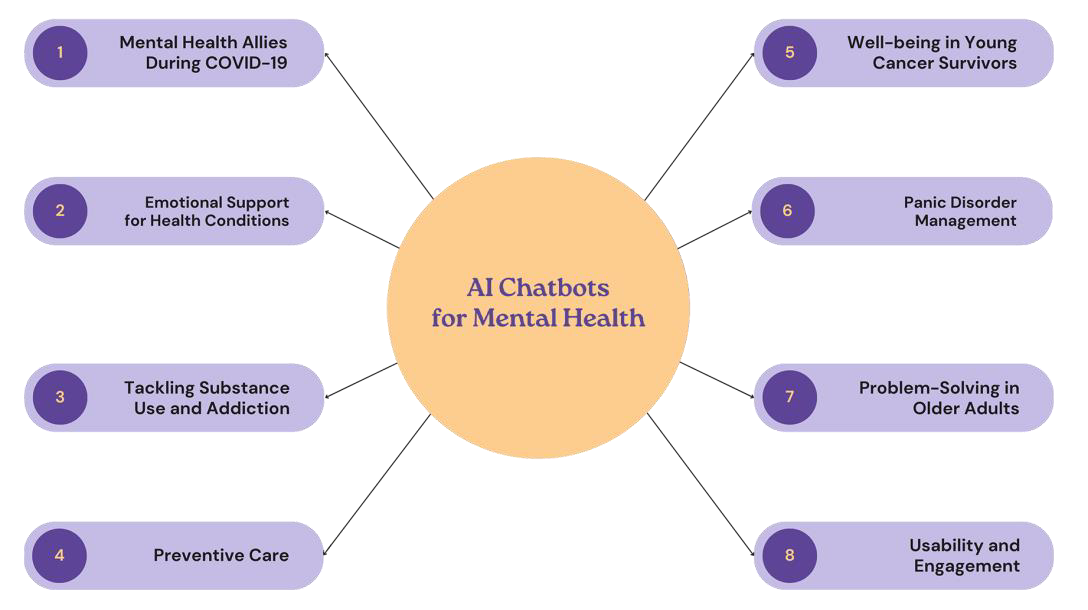
\includegraphics[width=0.75\linewidth]{mentalHealth.png}
    \caption{Različite primene chatbot-ova za mentalno zdravlje}
    \label{fig:placeholder}
\end{figure}

\subsection{Woebot Health}
Woebot je chatbot napravljen sa ciljem da omogući široj populaciji kvalitetnu psihološku podršku, a dostupan je i u vidu aplikacije za mobilni telefon.

\begin{figure}[h!]
    \centering
    
\includegraphics[width=0.5\linewidth]{WoeBot-A-Therapy-Chatbot.png}
    \caption{Woebot logo}
    \label{fig:placeholder}
\end{figure}

Woebot koristi stabla odlučivanja umesto generativnog LLM-a, ali koristi i NLP (Natural Language Processing) kako bi razgovor sa korisnicima bio tečan i prirodan. Kada uz pomoć NLP-a sistem prepozna nameru sa kojom mu korisnik piše, uz njenu pomoć bira već napisan i klinički odobren odgovor. Razlog zašto se ne koristi LLM jesu "halucinacije", netačne informacije predstavljene kao činjenice, koje se dešavaju usled prediktivne prirode ovakvih modela. Woebot sa druge strane mora biti potpuno deterministički, odnosno ne sme nikad davati nepredvidive savete pacijentima. Njegove razgovore pišu pisci u saradnji sa stručnjacima. Ipak, u pozadini se koriste LLM i drugi AI alati za analizu podataka u svrhe boljih odgovora i daljih kliničkih istraživanja. Woebot je takođe treniran da prepozna potencijalno zabrinjavajuć jezik i zatim pruži informacije o drugim vrstama pomoći koje su korisniku možda u tom momentu potrebnije. Naravno, Woebot održava strogu poverljivost i privatnost svojih korisnika za razliku od mnogih drugih chatbot-ova.\cite{woebot_health_responsible_ai}

Sve ove funkcionalnosti su tu kako bi Woebot mogao da se prepiše od strane lekara pacijentu kao "digitalni lek", pa tako osim što pruža pomoć onima koji nisu u mogućnosti da posete lekara, Woebot je tu i za one kojima trebaju dodatni razgovori, najčešće u pola noći ili tokom paničnih napada.

Ovaj chatbot, kreiran na Stanford univerzitetu 2017. godine, najviše je finansiran iz budžeta zdravstvenih i farmaceutskih organizacija kao i osiguravajućih kuća. Njegova svrha jeste isključivo da pomaže ljudima, a ne da zaradi na njima tako da su njegovi programeri takođe imali na umu da ne sme postojati rizik od razvijanja zavisnosti i emocionalne vezanosti. Razgovori su uglavnom kratki, do 10 minuta, a koriste se i principi osamostaljenja iz klasične psihoterapije gde je cilj da pacijent razvije sopstvene alate.

\section{Zaključak}

Chatbot-ovi predstavljaju moderni odgovor na krize društva u kome živimo. Njihova sposobnost da pruže anonimnu podršku  bez osude čini ih izuzetno efikasnim alatom za prevenciju i prvu psihološku pomoć. Međutim, ostavljaju prostora za eksploataciju ljudskih emocija i potreba.
AI Modeli Woebot i Replika su primeri kako veštačka inteligencija može biti dizajnirana da osnaži pojedinca. Međutim, iako upravo njihova osobina da se ponašaju kao idealni sagovornici pruža trenutnu utehu, dugoročno može oslabiti socijalne kapacitete korisnika za snalaženje u realnom svetu. 
Ovo implicira da izazov razvoja AI saputnika nije više tehničke prirode, već etičke: kako obezbediti pristupačnu podršku, bez daljeg skrnavljenja međuljudskih odnosa?
Chatbot-ovi nesumnjivo poseduju potencijal da budu dragocen saveznik u trenucima slabosti, ali ne smeju postati zamena za autentični ljudski kontakt.

\newpage
\printbibliography[title={Literatura}]

\end{document}
